\chapter{Manifolds}

We start with the definition of topological manifolds. We will later study the smooth manifolds that are of our main interest in this lecture. But first, we need to review some basic definition.

\begin{definition}[Hausdorff topological space]
	A set $ A $, along with a collection of subsets of $ A $ called $ \mathcal{T} \subset 2^A $, i.e. $ (A,\mathcal{T}) $ is called a topological space if we have
	\begin{enumerate}[(I)]
		\item $ \emptyset \in \mathcal{T} $ and $ A \in \mathcal{T} $.
		\item For any infinite collection $ \set{A_\alpha}_\alpha \subset \mathcal{T} $ we have
		\[ \bigcup_{\alpha} A_\alpha \in \mathcal{T}. \]
		\item For a finite collection $ \set{A_i}_{i \in I} $ where $ I = \set{1,2,\cdots,N} $ for some $ N \in \N $, we have
		\[ \bigcap_{i \in I} A_i \in \mathcal{T}. \]
		\item $ \forall x,y \in A $ there exists $ U,V \in \mathcal{T} $ such that $ x\in U $ and $ y \in V $ and we have $ U \cap V = \emptyset $.
	\end{enumerate}
\end{definition}


The following definition reviews the notion of second countable topological spaces.

\begin{definition}[Second countable topological spaces]
	Let $ (X,\mathcal{T}) $ be a topological space. This space is second countable if there exists an at most countable collection of sets $ \mathcal{B} \subset \mathcal{T} $ such that $ \forall U \in \mathcal{T} $ we have
	\[ U = \bigcup_{A \in \mathcal{B}} A. \]
	I.e. any open set in $ \mathcal{T} $ can be written as a union of sets in $ \mathcal{B} $
\end{definition} 

The last piece of definition that we need is the notion of locally Euclidean spaces.

\begin{definition}[Locally Euclidean topological spaces]
	Let $ (X,\mathcal{T}) $ be a topological space. We say $ X $ is locally Euclidean if $ \forall p \in X $, there exists an open neighborhood $ p \in U \in \mathcal{T}$ such that is homeomorphic to an \emph{open} subset of $ \R^n $. I.e. there is a homeomorphism $ \phi: U \to \R^n $. We call the pair $ (U,\phi:U\to\R^n) $ a \emph{chart}, $ U $ a \emph{coordinate neighborhood} or a \textbf{coordinate open set}, and $ \phi $ a \emph{coordinate map} or \emph{coordinate system} on $ U $. 
\end{definition}


\begin{definition}[Topological manifolds]
	A topological manifold is a Hausdorff, second countable topological space that is locally Euclidean space. It is said to be of dimension $ n $, if it is locally Euclidean of dimension $ n $.
\end{definition}


In the following section, we will review the notion of compatible charts which will be central to our study of manifolds. Assume we have two charts $ (U,\phi) $ and $ (V,\psi) $. Since $  U,V $ are open in $ M $ (the manifold), then $ U\cap V $ is open in $ U $ and $ V $. Furthermore, since $ \phi $ is a homeomorphism to an open subset of $ \R^n $ then $ \phi(U\cap V) $ and $ \psi(U\cap V) $ are also open. One way to show this, let $ \phi(U cap V) = B, \phi(U) = A, $ and $ A\backslash B = C $. We know that $  A $ is open, and $ B\cup C = A, B \cap C = \emptyset $. Then $ A $ being open implies $ B $ and $ C $ is open. Now we can make the following definition for $ C^\infty $-compatible maps.

\begin{definition}[$ C^\infty $ compatible maps]
	Let $ M $ be a topological manifold, where $ (U,\phi) $ and $ (V,\psi) $ are two charts. These charts are called $ C^\infty $-compatible if the maps
	\[ \phi\circ \inv{\psi} : \psi(U\cap V) \to \phi(U\cap V)\qquad \text{and} \qquad  \psi \circ\inv{\phi}: \phi(U \cap V) \to \psi(U\cap V),  \]
	are $ C^\infty $. These two maps are called \emph{transition functions} between charts. 
\end{definition}

\begin{remark}
	If two $ U,V $ in the definition above, i.e. $ U\cap V = \emptyset $, then they are automatically compatible.
\end{remark}

\begin{definition}[$ C^\infty $ atlas]
	Let $ M $ be a topological manifold. The collection of charts $ \mathcal{U} = \set{(U_\alpha, \phi_\alpha)} $ is called a $ C^\infty $ atlas, or simply an atlas if 
	\begin{itemize}
		\item all of the charts are pairwise $ C^\infty $ compatible,
		\item the charts cover the whole manifold, i.e. $ M = \bigcup_\alpha U_\alpha $.
	\end{itemize}
\end{definition}

\begin{lemma}
	Let $ \mathcal{A} = \set{(U_\alpha,\phi_\alpha)}_{\alpha \in I} $ be an atlas for the manifold $ M $. Let $ (V,\psi) $ and $ (W,\sigma) $ be two charts where both of them are compatible with the atlas $ \mathcal{A} $. Then these two charts are compatible with each other.
\end{lemma}

\begin{proof}
	We start by showing that $ \psi\circ \inv{\sigma} $ is $ C^\infty $ on $ V\cap W $. Let $ p \in V \cap W $. Then $ \exists \alpha \in I $ such that $ p \in U_\alpha $ for the chart $ (U_\alpha,\phi_\alpha) $. Then 
	\[ (\psi \circ \inv{\phi_\alpha})\circ (\phi_\alpha \circ \inv{\sigma}): \sigma(W\cap U_\alpha \cap V) \to \psi(W \cap U_\alpha \cap V) \]
	is $ C^\infty $ in $ \sigma(W\cap U_\alpha \cap V) $, because it is the composition of $ C^\infty $ maps. Call $ \mathbb{B}_\alpha  = W\cap U_\alpha \cap V $. Then what we have shows is simply $ \forall p \in V \cap W $, there exists an open set $ p \in \mathbb{B}_\alpha \subset V\cap W $ for $  \alpha \in I $ and the map $ \psi \circ \inv{\sigma}  $ is $ C^\infty $ in $ \mathbb{B}_\alpha $. Since this holds for every $ p \in V \cap W $ this proves that $ \psi\circ \inv{\sigma} $ is $ C^\infty $ on $ \sigma (V\cap W) $. Similarly, we can show $ \sigma \circ \inv{\psi} $ is $ C^\infty $ on $ \psi(V\cap W) $, and this completes the proof.
\end{proof}

\begin{remark}
	Note that in an equality like $ \psi \circ \inv{\sigma} =(\psi \circ \inv{\phi_\alpha})\circ (\phi_\alpha \circ \inv{\sigma}) $, two functions in the sides of the equality have different domains. So the equality sign here means that these two functions are equal on their common domain.
\end{remark}




\section{Solved Problems}

\begin{problem}[A $ C^\infty $ atlas on a circle (From W. Tu)]
	construct a $ C^\infty $ atlas for the unit circle $ S^1 $. 
\end{problem}
\begin{solution}
	The unit circle $ C^1 $ can be described as a set of points $ S^1 =  \set{e^{it}| t \in [0,2\pi]} $. Let $ U_1 $ and $ U_2 $ be two subsets of $ S^1 $ described as
	\[ U_1 = \set{e^{it}| t \in (-\pi,\pi)},\qquad U_2 = \set{e^{it}| t \in (0,2\pi)}. \]
	Consider the functions $ \phi_\alpha: U_\alpha \to \R $ for $ \alpha = 1,2 $ given by
	\begin{align*}
		&\phi_1(e^{it}) = t, \qquad -\pi<t<\pi,\\
		&\phi_2(e^{it}) = t, \qquad 0<t<2\pi.
	\end{align*}
	These functions are in fact different branches of the complex logarithm function $ 1/i\log(z) $, thus homeomorphisms onto their respective images. Thus $ \set{(U_1,\phi_1),(U_2,\phi_2)} $ is an atlas for $ S^1 $. To demonstrate the compatibility of these charts, we need to first calculate $ U_1 \cap U_2 $. This set has two connected components, i.e. $ U_1 \cap U_2 = A \sqcup B $ where $ \sqcup $ is used to demonstrate the disjoint union of $ A,B $. Explicitly, we can write
	\[ A = \set{e^{it}| t \in (-\pi,0)}, \qquad B = \set{e^{it}| t\in(0,\pi)}. \]
	First, we start with the function $ \phi_1 \circ \phi_2^{-1}: \underbrace{\phi_2(U_1\cap U_2)}_{(0,\pi)\sqcup (\pi,2\pi)} \to \underbrace{\phi_1(U_1\cap U_2)}_{(-\pi,0)\sqcup (0,\pi)} $. For this function we have
	\[ (\phi_1\circ\phi_2^{-1})(t) = \begin{cases}
		t \qquad &t\in(0,\pi),\\
		t - 2\pi \qquad &t\in(\pi,2\pi).
	\end{cases} \]
	Similarly, for $ \phi_2 \circ \phi_1^{-1}: \underbrace{\phi_1(U_1\cap U_2)}_{(-\pi,0)\sqcup (0,\pi)} \to \underbrace{\phi_2(U_1\cap U_2)}_{(0,\pi)\sqcup (\pi,2\pi)} $ we can write
	\[ (\phi_2\circ\phi_1^{-1})(t) = \begin{cases}
		t+2\pi \qquad &t\in(0,\pi),\\
		t \qquad &t\in(\pi,2\pi).
	\end{cases} \]
	\begin{figure}[h!]
	\centering

	
	
	\tikzset{every picture/.style={line width=0.75pt}} %set default line width to 0.75pt        
	
	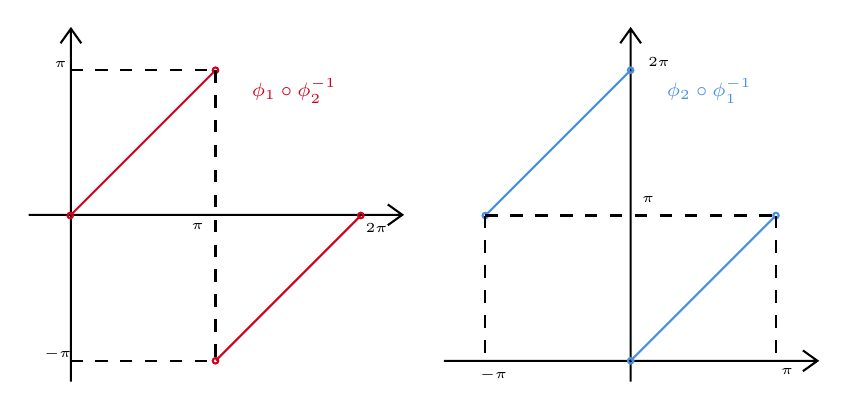
\begin{tikzpicture}[x=0.75pt,y=0.75pt,yscale=-1,xscale=1]
		%uncomment if require: \path (0,300); %set diagram left start at 0, and has height of 300
		
		%Shape: Axis 2D [id:dp031269396086308854] 
		\draw  (180,189.67) -- (360,189.67)(200.33,100) -- (200.33,270) (353,184.67) -- (360,189.67) -- (353,194.67) (195.33,107) -- (200.33,100) -- (205.33,107)  ;
		%Straight Lines [id:da8173483474090752] 
		\draw [color={rgb, 255:red, 208; green, 2; blue, 27 }  ,draw opacity=1 ][line width=0.75]    (200.24,189.76) -- (269.76,120.24) ;
		\draw [shift={(270,120)}, rotate = 315] [color={rgb, 255:red, 208; green, 2; blue, 27 }  ,draw opacity=1 ][line width=0.75]      (0, 0) circle [x radius= 1.34, y radius= 1.34]   ;
		\draw [shift={(200,190)}, rotate = 315] [color={rgb, 255:red, 208; green, 2; blue, 27 }  ,draw opacity=1 ][line width=0.75]      (0, 0) circle [x radius= 1.34, y radius= 1.34]   ;
		%Straight Lines [id:da7972743834901372] 
		\draw [color={rgb, 255:red, 208; green, 2; blue, 27 }  ,draw opacity=1 ][line width=0.75]    (270.24,259.76) -- (339.76,190.24) ;
		\draw [shift={(340,190)}, rotate = 315] [color={rgb, 255:red, 208; green, 2; blue, 27 }  ,draw opacity=1 ][line width=0.75]      (0, 0) circle [x radius= 1.34, y radius= 1.34]   ;
		\draw [shift={(270,260)}, rotate = 315] [color={rgb, 255:red, 208; green, 2; blue, 27 }  ,draw opacity=1 ][line width=0.75]      (0, 0) circle [x radius= 1.34, y radius= 1.34]   ;
		%Straight Lines [id:da11749218813373297] 
		\draw  [dash pattern={on 4.5pt off 4.5pt}]  (270,120) -- (270,260) ;
		%Shape: Axis 2D [id:dp7242837319994968] 
		\draw  (380,260) -- (560,260)(470,100) -- (470,270) (553,255) -- (560,260) -- (553,265) (465,107) -- (470,100) -- (475,107)  ;
		%Straight Lines [id:da7954245800299584] 
		\draw [color={rgb, 255:red, 74; green, 144; blue, 226 }  ,draw opacity=1 ][line width=0.75]    (400.24,189.76) -- (469.76,120.24) ;
		\draw [shift={(470,120)}, rotate = 315] [color={rgb, 255:red, 74; green, 144; blue, 226 }  ,draw opacity=1 ][line width=0.75]      (0, 0) circle [x radius= 1.34, y radius= 1.34]   ;
		\draw [shift={(400,190)}, rotate = 315] [color={rgb, 255:red, 74; green, 144; blue, 226 }  ,draw opacity=1 ][line width=0.75]      (0, 0) circle [x radius= 1.34, y radius= 1.34]   ;
		%Straight Lines [id:da15608839189923596] 
		\draw [color={rgb, 255:red, 74; green, 144; blue, 226 }  ,draw opacity=1 ][line width=0.75]    (470.24,259.76) -- (539.76,190.24) ;
		\draw [shift={(540,190)}, rotate = 315] [color={rgb, 255:red, 74; green, 144; blue, 226 }  ,draw opacity=1 ][line width=0.75]      (0, 0) circle [x radius= 1.34, y radius= 1.34]   ;
		\draw [shift={(470,260)}, rotate = 315] [color={rgb, 255:red, 74; green, 144; blue, 226 }  ,draw opacity=1 ][line width=0.75]      (0, 0) circle [x radius= 1.34, y radius= 1.34]   ;
		%Straight Lines [id:da8863860410352722] 
		\draw  [dash pattern={on 4.5pt off 4.5pt}]  (400,190) -- (400,260) ;
		%Straight Lines [id:da8092780134149673] 
		\draw  [dash pattern={on 4.5pt off 4.5pt}]  (540,190) -- (540,260) ;
		%Straight Lines [id:da9907647632614371] 
		\draw  [dash pattern={on 4.5pt off 4.5pt}]  (400,190) -- (540,190) ;
		%Straight Lines [id:da6719155425075689] 
		\draw  [dash pattern={on 4.5pt off 4.5pt}]  (200,260) -- (270,260) ;
		%Straight Lines [id:da26461137148185054] 
		\draw  [dash pattern={on 4.5pt off 4.5pt}]  (200,120) -- (270,120) ;
		
		% Text Node
		\draw (257,192.4) node [anchor=north west][inner sep=0.75pt]  [font=\tiny]  {$\pi $};
		% Text Node
		\draw (286,122.4) node [anchor=north west][inner sep=0.75pt]  [font=\scriptsize,color={rgb, 255:red, 208; green, 2; blue, 27 }  ,opacity=1 ]  {$\phi _{1} \circ \phi _{2}^{-1}$};
		% Text Node
		\draw (341,192.4) node [anchor=north west][inner sep=0.75pt]  [font=\tiny]  {$2\pi $};
		% Text Node
		\draw (396,262.4) node [anchor=north west][inner sep=0.75pt]  [font=\tiny]  {$-\pi $};
		% Text Node
		\draw (486,122.4) node [anchor=north west][inner sep=0.75pt]  [font=\scriptsize,color={rgb, 255:red, 74; green, 144; blue, 226 }  ,opacity=1 ]  {$\phi _{2} \circ \phi _{1}^{-1}$};
		% Text Node
		\draw (541,262.4) node [anchor=north west][inner sep=0.75pt]  [font=\tiny]  {$\pi $};
		% Text Node
		\draw (474,179.4) node [anchor=north west][inner sep=0.75pt]  [font=\tiny]  {$\pi $};
		% Text Node
		\draw (477,112.4) node [anchor=north west][inner sep=0.75pt]  [font=\tiny]  {$2\pi $};
		% Text Node
		\draw (191,114.4) node [anchor=north west][inner sep=0.75pt]  [font=\tiny]  {$\pi $};
		% Text Node
		\draw (186,252.4) node [anchor=north west][inner sep=0.75pt]  [font=\tiny]  {$-\pi $};
		
		
	\end{tikzpicture}
\end{figure}

\end{solution}

\begin{observation}
	I was thinking about my solution to the problem above, and I thought it is wrong, as I was thinking that the function $ \phi_1 $ is not homeomorphism as it is not continuous. But the point that I was missing is that this function is indeed continuous on its domain and the point of discontinuity (i.e. $ x = \pi $) is not in the domain. 
\end{observation}

\begin{problem}{Another $ C^\infty $ atlas on a circle}
	In the previous problem, we constructed an atlas for a unit circle siting in the complex plane. In this problem we are going to construct a different atlas for a unit circle siting in the $ x-y $ plane. The following diagram are the charts for this unit circle. Write these charts explicitly and check if they are pairwise compatible.
	\begin{figure}[h!]
	
	
	\centering
	\tikzset{every picture/.style={line width=0.75pt}} %set default line width to 0.75pt        
	
	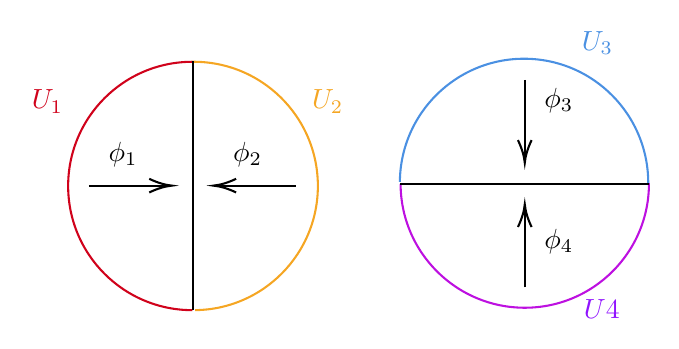
\begin{tikzpicture}[x=0.75pt,y=0.75pt,yscale=-1,xscale=1]
		%uncomment if require: \path (0,300); %set diagram left start at 0, and has height of 300
		
		%Shape: Arc [id:dp023481932229717062] 
		\draw  [draw opacity=0] (199.83,250) .. controls (199.83,250) and (199.83,250) .. (199.83,250) .. controls (199.83,250) and (199.83,250) .. (199.83,250) .. controls (166.79,250) and (140,223.21) .. (140,190.17) .. controls (140,157.12) and (166.79,130.33) .. (199.83,130.33) -- (199.83,190.17) -- cycle ; \draw  [color={rgb, 255:red, 208; green, 2; blue, 27 }  ,draw opacity=1 ] (199.83,250) .. controls (199.83,250) and (199.83,250) .. (199.83,250) .. controls (199.83,250) and (199.83,250) .. (199.83,250) .. controls (166.79,250) and (140,223.21) .. (140,190.17) .. controls (140,157.12) and (166.79,130.33) .. (199.83,130.33) ;  
		%Shape: Arc [id:dp8279857043077765] 
		\draw  [draw opacity=0] (199.83,130.33) .. controls (199.83,130.33) and (199.83,130.33) .. (199.83,130.33) .. controls (232.88,129.98) and (259.95,156.47) .. (260.31,189.52) .. controls (260.67,222.56) and (234.17,249.64) .. (201.13,249.99) -- (200.48,190.16) -- cycle ; \draw  [color={rgb, 255:red, 245; green, 166; blue, 35 }  ,draw opacity=1 ] (199.83,130.33) .. controls (199.83,130.33) and (199.83,130.33) .. (199.83,130.33) .. controls (232.88,129.98) and (259.95,156.47) .. (260.31,189.52) .. controls (260.67,222.56) and (234.17,249.64) .. (201.13,249.99) ;  
		%Shape: Arc [id:dp2277450931666709] 
		\draw  [draw opacity=0] (299.82,188.21) .. controls (299.82,188.21) and (299.82,188.21) .. (299.82,188.21) .. controls (300.08,155.16) and (327.08,128.59) .. (360.13,128.86) .. controls (393.17,129.12) and (419.75,156.12) .. (419.48,189.17) -- (359.65,188.69) -- cycle ; \draw  [color={rgb, 255:red, 74; green, 144; blue, 226 }  ,draw opacity=1 ] (299.82,188.21) .. controls (299.82,188.21) and (299.82,188.21) .. (299.82,188.21) .. controls (300.08,155.16) and (327.08,128.59) .. (360.13,128.86) .. controls (393.17,129.12) and (419.75,156.12) .. (419.48,189.17) ;  
		%Shape: Arc [id:dp16056893747855794] 
		\draw  [draw opacity=0] (419.83,188.83) .. controls (419.83,188.83) and (419.83,188.83) .. (419.83,188.83) .. controls (419.93,221.88) and (393.21,248.74) .. (360.17,248.83) .. controls (327.12,248.93) and (300.26,222.21) .. (300.17,189.17) -- (360,189) -- cycle ; \draw  [color={rgb, 255:red, 189; green, 16; blue, 224 }  ,draw opacity=1 ] (419.83,188.83) .. controls (419.83,188.83) and (419.83,188.83) .. (419.83,188.83) .. controls (419.93,221.88) and (393.21,248.74) .. (360.17,248.83) .. controls (327.12,248.93) and (300.26,222.21) .. (300.17,189.17) ;  
		%Straight Lines [id:da9947609889928073] 
		\draw    (150,190) -- (188,190) ;
		\draw [shift={(190,190)}, rotate = 180] [color={rgb, 255:red, 0; green, 0; blue, 0 }  ][line width=0.75]    (10.93,-3.29) .. controls (6.95,-1.4) and (3.31,-0.3) .. (0,0) .. controls (3.31,0.3) and (6.95,1.4) .. (10.93,3.29)   ;
		%Straight Lines [id:da6553860547904606] 
		\draw    (212,190) -- (250,190) ;
		\draw [shift={(210,190)}, rotate = 0] [color={rgb, 255:red, 0; green, 0; blue, 0 }  ][line width=0.75]    (10.93,-3.29) .. controls (6.95,-1.4) and (3.31,-0.3) .. (0,0) .. controls (3.31,0.3) and (6.95,1.4) .. (10.93,3.29)   ;
		%Straight Lines [id:da19474028508083085] 
		\draw    (360,139) -- (360,177) ;
		\draw [shift={(360,179)}, rotate = 270] [color={rgb, 255:red, 0; green, 0; blue, 0 }  ][line width=0.75]    (10.93,-3.29) .. controls (6.95,-1.4) and (3.31,-0.3) .. (0,0) .. controls (3.31,0.3) and (6.95,1.4) .. (10.93,3.29)   ;
		%Straight Lines [id:da648683487634115] 
		\draw    (360,239) -- (360,201) ;
		\draw [shift={(360,199)}, rotate = 90] [color={rgb, 255:red, 0; green, 0; blue, 0 }  ][line width=0.75]    (10.93,-3.29) .. controls (6.95,-1.4) and (3.31,-0.3) .. (0,0) .. controls (3.31,0.3) and (6.95,1.4) .. (10.93,3.29)   ;
		%Straight Lines [id:da9130830416071034] 
		\draw    (200,130) -- (200,250) ;
		%Straight Lines [id:da1322223309435544] 
		\draw    (420,189) -- (300,189) ;
		
		% Text Node
		\draw (121,142.4) node [anchor=north west][inner sep=0.75pt]  [color={rgb, 255:red, 208; green, 2; blue, 27 }  ,opacity=1 ]  {$U_{1}$};
		% Text Node
		\draw (256,142.4) node [anchor=north west][inner sep=0.75pt]  [color={rgb, 255:red, 245; green, 166; blue, 35 }  ,opacity=1 ]  {$U_{2}$};
		% Text Node
		\draw (386,114.4) node [anchor=north west][inner sep=0.75pt]  [color={rgb, 255:red, 74; green, 144; blue, 226 }  ,opacity=1 ]  {$U_{3}$};
		% Text Node
		\draw (387,243.4) node [anchor=north west][inner sep=0.75pt]  [color={rgb, 255:red, 144; green, 19; blue, 254 }  ,opacity=1 ]  {$U4$};
		% Text Node
		\draw (158,167.4) node [anchor=north west][inner sep=0.75pt]    {$\phi _{1}$};
		% Text Node
		\draw (218,167.4) node [anchor=north west][inner sep=0.75pt]    {$\phi _{2}$};
		% Text Node
		\draw (368,141.4) node [anchor=north west][inner sep=0.75pt]    {$\phi _{3}$};
		% Text Node
		\draw (368,209.4) node [anchor=north west][inner sep=0.75pt]    {$\phi _{4}$};
		
		
	\end{tikzpicture}
\end{figure}

\FloatBarrier
\end{problem}
\begin{solution}
	The explicit formulas for the charts depicted above is as following
	\[ (U_1, \phi_1:U_1\to \R),(U_2, \phi_2:U_2\to \R), (U_3, \phi_3:U_3\to \R),(U_4, \phi_4:U_4\to \R), \]
	where we have
	\[ \phi_1(x,y) = y,\qquad  \phi_2(x,y) = y, \qquad \phi_3(x,y) = x, \qquad \phi_4(x,y) = x. \]
	Note that although some of the functions above might have a same formula, but they are different functions as they have different domains. To show that these functions are pairwise compatible, we start by noting that since $ U_1 \cap U_2 = \emptyset $, thus $ (U_1,\phi_1) $ and $ (U_2,\phi_2) $ are compatible. With the same reasoning, the charts $ (U_3,\phi_3) $ and $ (U_4,\phi_4) $ are compatible. Now, we want to show that $ (U_1,\phi_1) $ is compatible with $ (U_3,\phi_3) $. We need to show that 
	\[ \phi_1 \circ \inv{\phi_3}: \underbrace{\phi_3(U_1\cap U_3)}_{(-1,0)} \to \underbrace{\phi_1(U_1\cap U_3)}_{(0,1)}\quad \text{and} \quad \phi_3\circ \inv{\phi_1}:\underbrace{\phi_1(U_1\cap U_3)}_{(0,1)} \to \underbrace{\phi_3(U_1\cap  U_3)}_{(-1,0)} \]
	are $ C^\infty $. To write them explicitly, we have
	\[ (\phi_1 \circ \inv{\phi_3})(x) = \phi_1(x,\sqrt{1-x^2}) = \sqrt{1-x^2}.  \]
	Also
	\[ (\phi_3 \circ \inv{\phi_1})(x) = \phi_3(-\sqrt{1-x^2},x) = -\sqrt{1-x^2}. \]
	We can see that both of these functions are $ C^\infty $ in their domain. Now, for the charts $ (U_1, \phi_1) $ and $ (U_4,\phi_4) $ need to show
	\[ \phi_1 \circ \inv{\phi_4}:\underbrace{ \phi_4(U_1\cap U_4)}_{(-1,0)} \to \underbrace{\phi_1(U_1\cap U_4)}_{(-1,0)} \qquad \text{and} \qquad \phi_4\circ \inv{\phi_1}: \underbrace{\phi_1(U_1\cap U_4)}_{(-1,0)} \to  \underbrace{\phi_4(U_1\cap U_4)}_{(-1,0)} \]
	are $ C^\infty $ in their domain. Explicitly, we have
	\[ (\phi_1 \circ \inv{\phi_4})(x) = -\sqrt{1 -x^2}, \qquad (\phi_4\circ \inv{\phi_1})(x) = -\sqrt{1-x^2}.\]
	With the same strategy, we can show that this collection of charts indeed makes a $ C^\infty $ atlas for the unit circle in $ x-y $ plane.
\end{solution}


\begin{problem}[The real line with two origins (from W. Tu)]
	Let $ A $ and $ B $ be two points not on the real line $ \R $. Consider the set $ S = (\R - \set{0}) \cup \set{A,B} $. For nay two positive real numbers $ c,d $, define 
	\[ I_A(-c,d) = (-c,0) \cup \set{A} \cap (0,d) \]
	and similarly for $ I_B(-c,d) $, with $ B $ instead of $ A $. Define a topology on $ S $ as follows: On $ (\R - \set{0}) $, use the subspace topology inherited from $ \R $, with open intervals as a basis. A basis of neighborhoods at $ A $ is the set $ \set{I_A(-c,d)\ |\ c,d > 0} $; similarly, a basis of neighborhoods at $ B $ is $ \set{I_B(-c,d)\ |\ c,d < 0} $.
	\begin{enumerate}[(a)]
		\item Prove that the map $ h: I_A(-c,d) \to (-c,d) $ defined by
		\[ h(x) = x \]
	\end{enumerate}
\end{problem}